%%%%%%%%%%%%%%%%%%%%%%%%%%%%%%%%%%%%%%%%%
%%% WP01
%%%%%%%%%%%%%%%%%%%%%%%%%%%%%%%%%%%%%%%%%

\tsubsubsection{WP2 - Access to RI for Physics}

%%%%%%%%%%%%%%%%%%%%%%%%%%%%%%%%%%%%%%%%%
%%% Section content, please change!
%%%%%%%%%%%%%%%%%%%%%%%%%%%%%%%%%%%%%%%%%

\subsubsection*{Overview and Goals}

\begin{table}[H]
    \renewcommand{\arraystretch}{1.50}		
    \footnotesize   
    \begin{tabular}{*{3}{|p{0.10\textwidth}}|l|}
        \hline
        \rowcolor{mygray} \multicolumn{4}{|c|}{\textit{\color{white}Work Package Summary}} \\
        \hline
        \rowcolor{mylightergray} \textit{WP No.} & \cellcolor{white} 02 & \textit{Title of WP} & \cellcolor{white} TA1/VA1: RIs for Nuclear Physics \\
        \hline
        \rowcolor{mylightergray} \textit{Start} & \cellcolor{white} M1 & \textit{End} & \cellcolor{white} M48 \\
        \hline
        \rowcolor{mylightergray} \multicolumn{4}{|p{0.978\textwidth}|}{\textit{Participating Organisations}} \\
        \hline
        \multicolumn{4}{|p{0.978\textwidth}|}{
            \hspace*{-0.75cm} 
            \begin{minipage}[t]{\textwidth}
    			\begin{itemize}
    			    \item WP Leader: 5. IFJ PAN
    				\item Participants: INFN, GANIL, CERN, IFJ-PAN, CNRS, UNIWARSAW, GSI, IFIN-HH, USE, Atomki, JYU, UMCG, UMIL, PSI
    			\end{itemize} 
    			\vspace*{0.10em}
			\end{minipage}
        } \\
        \hline
    \end{tabular}
    \vspace{0.5em}\vfill
    \begin{tabular}{|p{0.978\textwidth}|}
        \hline
        \rowcolor{mylightergray} \textit{Goals} \\
        \hline
        \rowcolor{white} 
        \hspace*{-0.75cm} 
        \begin{minipage}[t]{\textwidth}
        {\leftskip=15pt
        The goal of the work-package is the access provision, complemented by improved access services, to Research Infrastructures (RIs) for nuclear (fundamental and applied) physics experiments and related theoretical support.
    		\begin{itemize}
    		    \item Task 1: TA to RIs delivering Stable Ion Beams, coordinated by JYFL Jyvaskyla;
    			\item Task 2: TA to RIs delivering Radioactive Ion Beams (RIB), coordinated by ALTO IJCLab Orsay;
			    \item Task 3: TA to RIs delivering Neutron Beams, coordinated by n-TOF CERN.
                    \item Task 4: VA to RIs for theoretical support for experiments 
                    \item Task 5: Service improvements , coordinaed by GSI
    		\end{itemize} 
    		\vspace*{0.10em}
            }
		\end{minipage}        
        \\
        \hline
    \end{tabular}
    \vspace{0.5em}\vfill
    \resizebox{\textwidth}{!}{%
    \begin{tabular}{|p{0.15\textwidth}|*{7}{>{\centering\arraybackslash}p{0.11\textwidth}|}}
        \hline    
        \rowcolor{mylightergray} \textit{Participant number} & \textit{1} & \textit{2} & \textit{3} & \textit{4} & \textit{5}  & \textbf{6} & \textbf{7}\\
        \hline
        \rowcolor{white} \cellcolor{mylightergray}\textit{Participant short name} & INFN & GANIL & CERN & IFJ-PAN & CNRS & UNIWARSAW & GSI \\
        \hline
        \rowcolor{white} \cellcolor{mylightergray}\textit{PM per participant} & 45.5 & 12 & - & - & 10 & 24 & 43 \\
        \hline 
        \hline    
        \rowcolor{mylightergray} \textit{Participant number} & \textit{8} & \textit{9} & \textit{10} & \textit{11} & \textit{12} & \textbf{13} & \textbf{14}\\
        \hline
        \rowcolor{white} \cellcolor{mylightergray}\textit{Participant short name} & IFIN-HH & USE & Atomki & JYU & UMCG & UMIL & PSI \\
        \hline
        \rowcolor{white} \cellcolor{mylightergray}\textit{PM per participant~\footnotemark} & 4 & 52.8 & 8 & 12.5 & 12 & 40.8 & 3 \\
        \hline 
    \end{tabular}
    }
\end{table}
\footnotetext{the PM figures correspond to the full duration of the project.}

\subsubsection*{Status}


In P2, all WP2 TA facilities have been very successful in achieving the objective of promoting and facilitating access to the users. Overall, approximately 23 000 Access Units, which represents  78\% of the total number of Access Units promised in the GA, were provided in P2 of the project. 
%Thus, it can be deduced 
Considering also the access provided in RP1, 
an average of around 130\% of the promised AUs have been delivered from the beginning of the project. The costs of the additional beam hours were covered by the local budget of the facilities. The distribution of the access units for each TA facility, declared for the whole project, provided in P2 and provided since beginning of the project, is shown in Fig.~\ref{fig:WP2_AU_statistics}.

\begin{figure}[!h]
    \centering
    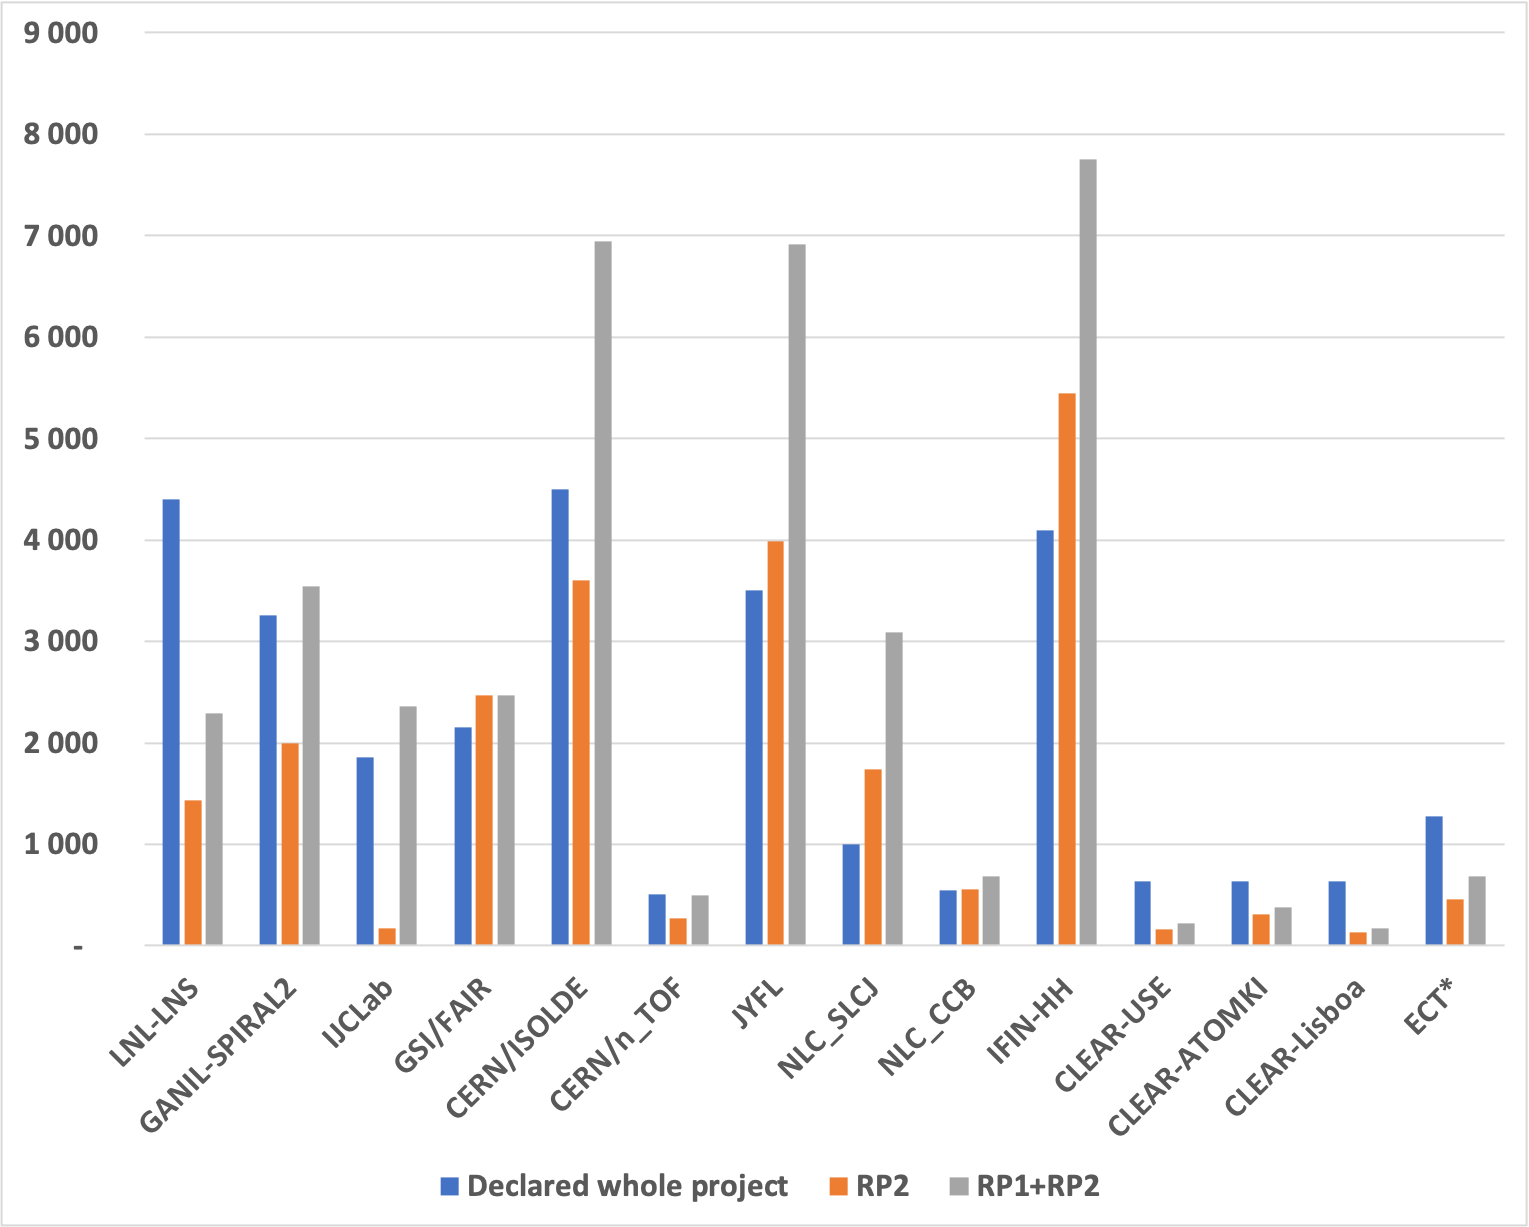
\includegraphics[width=0.8\linewidth]{graphics/WP2_AU_statistics.png}
    \caption{Distribution of the Access Units (hours of the beam time in the case of the beam facilities, or days of visits in the case of ECT*) provided within WP2 facilities in P2}
    \label{fig:WP2_AU_statistics}
\end{figure}

In P2, 194 TA projects were supported: 86 projects in Task 2.1 (Stable ion beams), 82 projects in Task 2.2 (Radioactive Ion beams), 11 projects in Task 2.3 (Neutron beams) and 11 projects for the TA access to the theory center ECT* (cf. Fig.~\ref{fig:WP2_projects}).  In addition, the facilities have exhausted in P2 28\% (which makes 45\% for both P1 and P2) of the allocated Travel and Subsistence (T\&S) funding, supporting traveling expenses and visits of 840 users (with approximately 30\% of female scientists) to prepare and develop instrumentation prior to the actual delivery of the beam, to run the experiments, or visit the theory center ECT*. Details are shown in the Figs.~\ref{fig:WP2_users_per_country} and~\ref{fig:WP2_users_men_women}. 

\begin{figure}[!h]
    \centering
    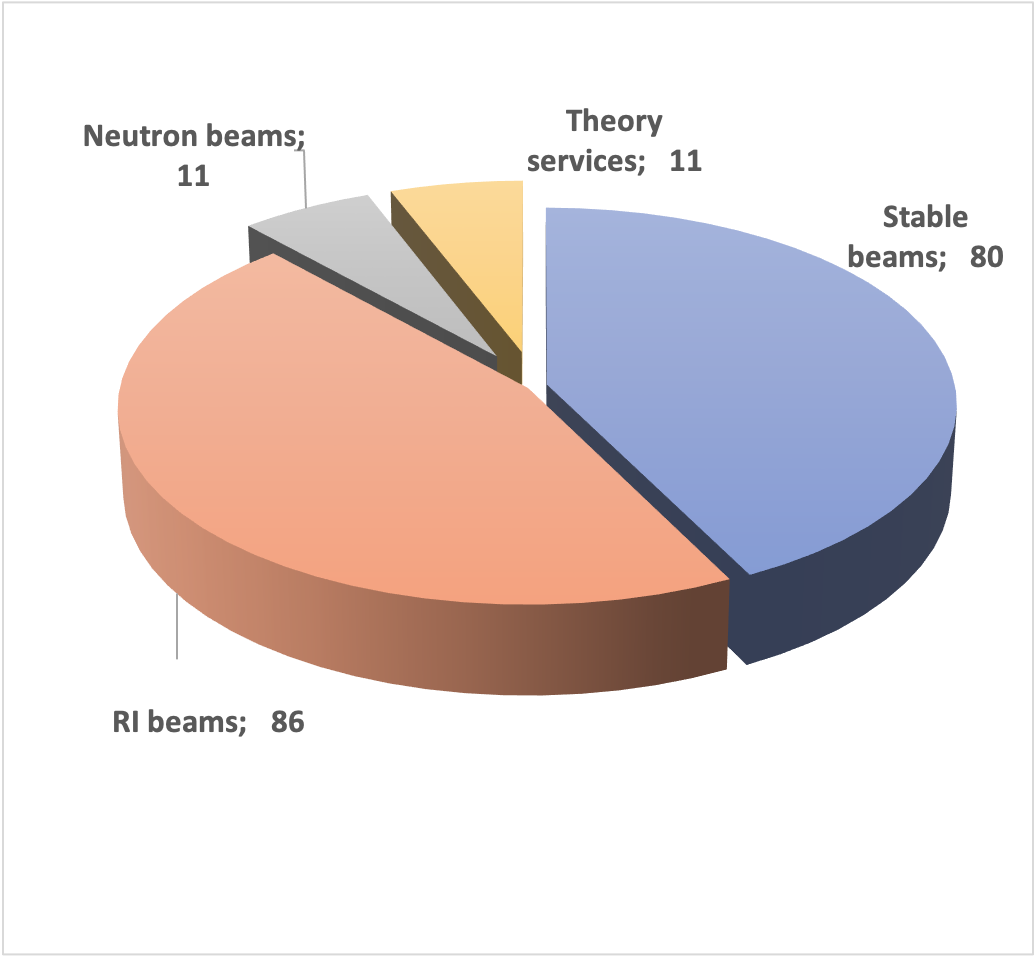
\includegraphics[width=0.95\linewidth]{graphics/WP2_projects.png}
    \caption{Left: TA Projects realized in P2 in different WP2 tasks. Right: Access Units used in P2 in different WP2 tasks.}
    \label{fig:WP2_projects}
\end{figure}


\begin{figure}[!h]
    \centering
    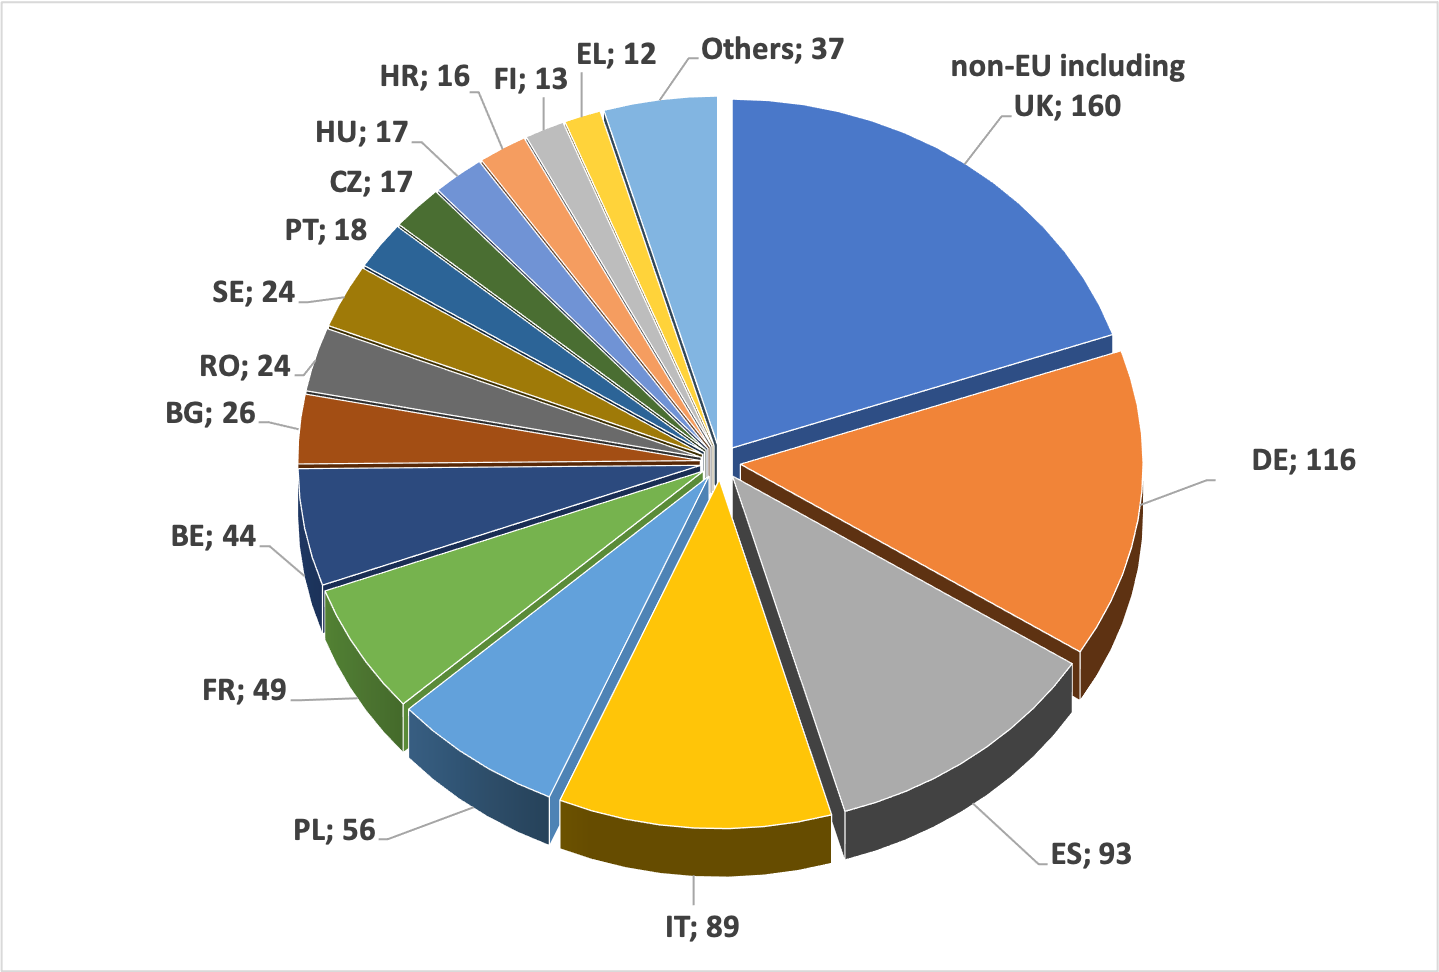
\includegraphics[width=1.0\linewidth]{graphics/WP2_users_per_country.png}
    \caption{Geographical distribution of TA users' home institutions in WP2 during P2.}
    \label{fig:WP2_users_per_country}
\end{figure}

\begin{figure}[!h]
    \centering
    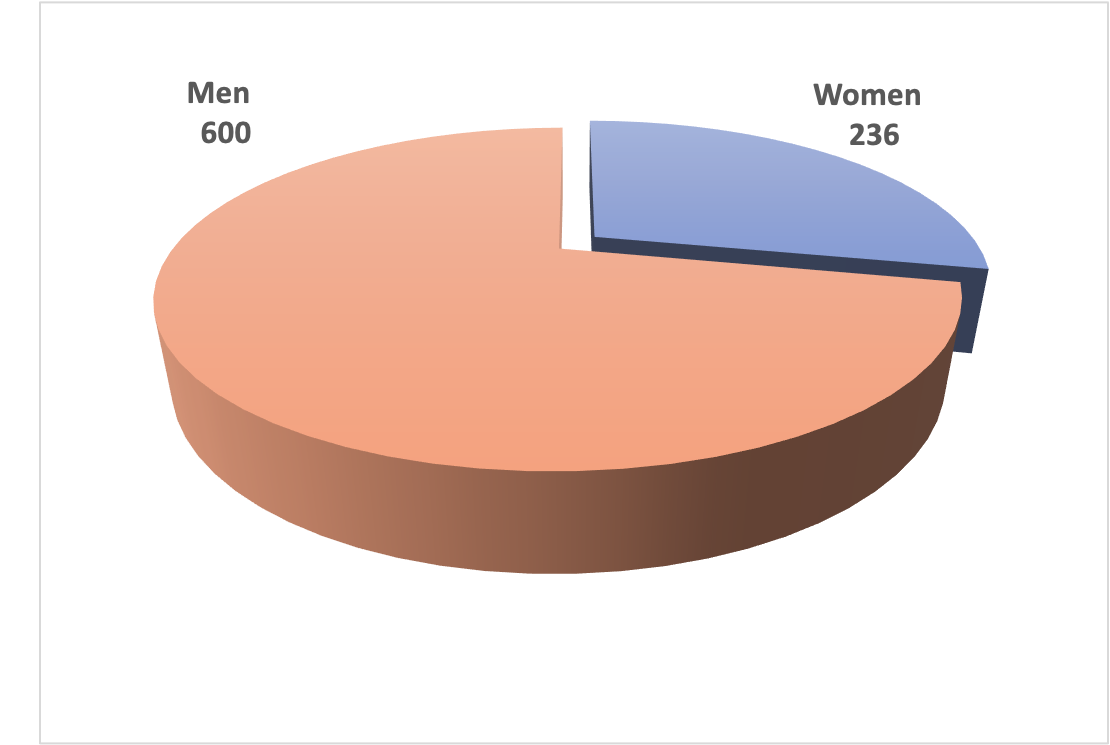
\includegraphics[width=0.6\linewidth]{graphics/WP2_users_men_women.png}
    \caption{Female vs. male distribution of TA users in WP2 during P2.}
    \label{fig:WP2_users_men_women}
\end{figure}


The activities planned in P2 for Service Improvement, related to streamlined and remote access, targets for high intense beams, biomedical applications, improving ion beam services and optimal employment of traveling gamma-ray detectors, have been progressing well. 

The synergy between theory and experiments has been secured by the TA offered at the ECT* center, where 11 events were organized, aimed at 
discussing hot topics in the field of nuclear structure and reactions
(microscopic optical potentials, strangeness in nuclear reactions, nuclear theory and reactions for astrophysics, hadron tomography, neutrino interactions, electric dipole moments,  and machine learning). 

Moreover, the new facility (Theo4Exp) offering VA to theoretical tools accessible via user-friendly web pages, to help preparing and interpreting experiments, has been successfully installed and started delivering access.
\subsubsection*{Progress per Task}
\subparagraph{Task 2.1: Stable Ion Beams} \mbox{}

%\todo{Briefly explain the progress of the task in context to the DoA.}

Period 2 has proven to be an extremely busy one for the Stable Ion Beam facilities of Task 2.1. All eight facilities (including consortia) have supported multiple experiments with a very high level of success. A total of 86 were supported in P2.

Whilst still performing the “traditional” forefront experiments in fundamental nuclear physics research, the program of science covered by the Stable Ion Beam facilities is very broad and multidisciplinary. Nuclear and accelerator-based techniques are being also used to address a variety of topics, 
%as far 
ranging from radiation shielding for lunar habitats (GSI-FAIR), radiation effects in 2D Nanostructures (GANIL), effects of heavy ion radiation on cells (GSI-FAIR and GANIL), to thin film elemental characterisation for photovoltaic cells (CLEAR – IST), improved processes for purification of phosphogypsum (CLEAR – IST), assessment of the impact of dumping of radioactive materials in the Baltic Sea region (CLEAR – CNA) and analysis of air quality in the city of Naples (CLEAR – ATOMKI).

It should be noted that a number of experiments which highlight the importance to the community of having a large range of facilities of different scale, offering different ion beams and techniques, with efficient and flexible access available. Novel $^3$He and $^4$He targets, made by magnetron sputtering and trapped in a suitable substrate, were characterised at \textbf{CLEAR-CNA} and subsequently used in fundamental nuclear science experiments at other facilities. For instance, the $^4$He targets were used to study elastic $\alpha$-scattering on heavy nuclei, relevant for nuclear astrophysics, and the $^3$He targets were to be used in the measurement of the lifetime of a subthreshold state in $^{15}$O, produced by neutron transfer from an $^{16}$O beam, using apparta (AGATA and SAURON) installed at INFN-LNL. 
%The $^{15}$O will be produced by neutron transfer to the $^3$He target from an $^{16}$O beam. 
At GANIL, experiments were made to assess the performance of thin, electrodeposited targets for future studies of Superheavy Elements (SHE) using high intensity ion beams. At \textbf{CLEAR-IST}, self-supporting $^{208}$Pb targets were characterised in order to reduce uncertainties in the analysis of Coulomb breakup experiments (to investigate $^6$He, for example). \textbf{CLEAR-ATOMKI}  characterised the tracking capability and sensitivity of detectors which will be used in a forthcoming experiment at the n$\_$TOF neutron irradiation facility at CERN. At \textbf{ALTO}, an in-beam test was made to investigate the high-rate performance of the detectors and read-out chain which will form part of the G-NUMEN gamma-array demonstrator. In future, the NUMEN experiment will be focused on Nuclear Matrix Elements for neutrinoless double beta decay. 

At \textbf{GANIL} eight stable ion beam projects were carried out, supported by 1448 hours of beam time. 

At \textbf{GSI/FAIR}, the NUSTAR collaboration carried out ten experiments during RP2, exploiting 1217 Access Units.  

At the \textbf{IFIN-HH} 24 experimental groups were supported and received 5450 hours of beam time. Data analysis is ongoing for most groups, but several have already published or submitted their results for publication. 

At \textbf{JYFL}, fourteen stable ion beam experiments were supported during the reporting period. The experiments were granted a total of 3096 hours of beam time access. Aside from one experiment which used the TOSCA two-arm time-of-flight spectrometer to study fission dynamics at the Large Scattering Chamber, the recoil separators RITU and MARA 
were employed
to study various aspects of nuclear structure physics and reaction dynamics, in particular Multi-Nucleon Transfer reactions. The efficiency of performing campaigns at the separators, which can house the JUROGAM3 array of germanium detectors at their target positions, has been enhanced by the use of a gantry which allows the array to move from one separator to another within hours (see Fig.~\ref{fig:Jurogam3}). This removes the need to un-bias the detectors before moving the array, which previously resulted in a need to anneal the detectors to repair radiation damage. The latter procedure can take weeks-months. 

\begin{figure}[!h]
    \centering
    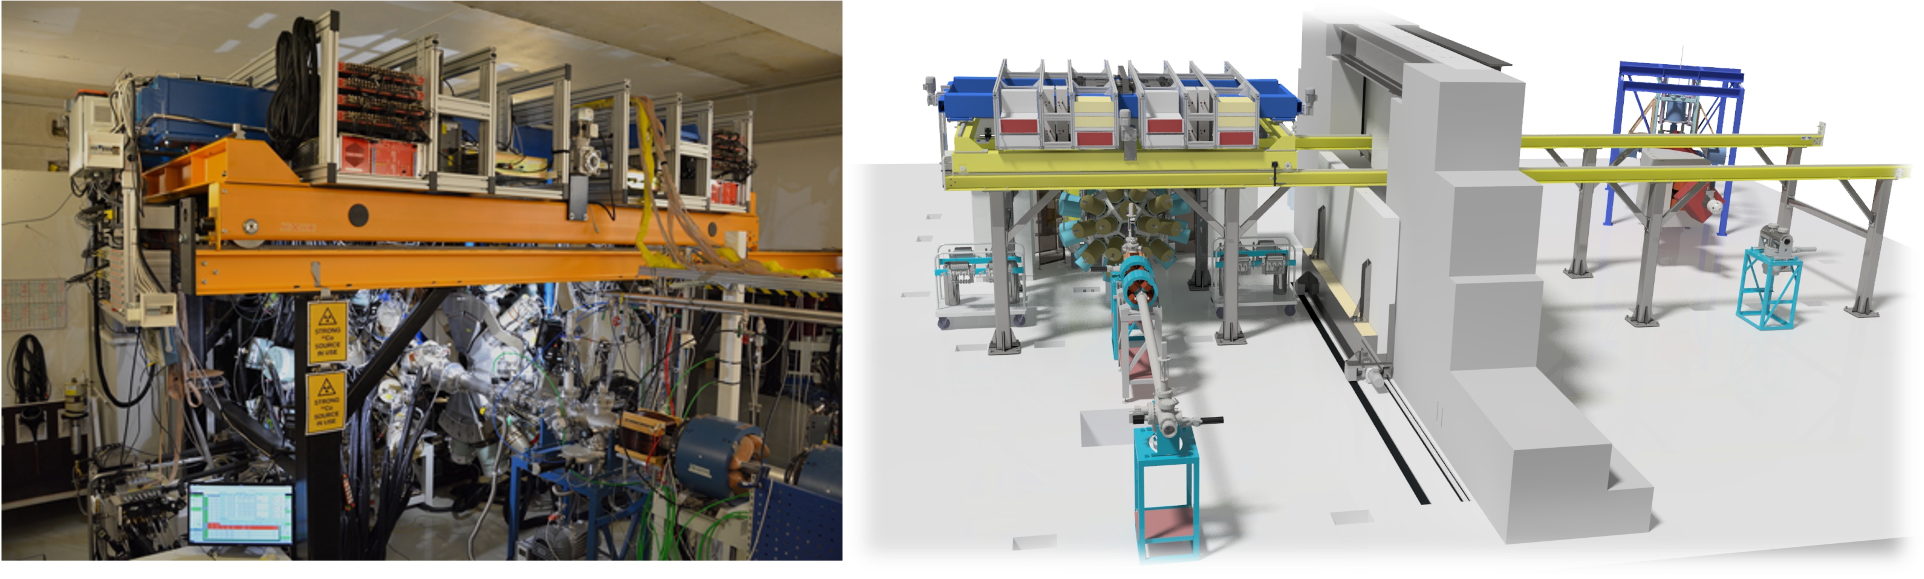
\includegraphics[width=1.0\linewidth]{graphics/Jurogam3.png}
    \caption{The JUROGAM3 array at the target position of the MARA recoil separator and the gantry system to allow rapid relocation of the array to the sister separator, RITU.}
    \label{fig:Jurogam3}
\end{figure}

At \textbf{INFN-LNL}, a total of ten experiments were supported during P2,  using 1431 access units. The experiments exploited the European AGATA gamma-ray tracking array (see Fig.~\ref{fig:AGATA_LNL}) in various configurations with ancillary detectors. Using AGATA-SPIDER, a number of Coulomb excitation experiments were performed to study several aspects of nuclear structure, such as the emergence of collectivity near $^{60}$Ni (experiment 23.008) and the interpretation of the structure of excited 0$^+$ states in $^{106}$Pd (experiment 23.054). AGATA-PRISMA was used, along with RDDS and DSAM techniques, to measure lifetimes in $^{50-52}$Ca and $^{46-48}$Ar, aiming to understand shell evolution close to N=28 and Z=20 (experiment 22.81). The same devices were used to measure Multi-Nucleon Transfer (MNT) reactions. 
 Other devices combined with AGATA for experiments were AGATA-SAURON, AGATA-EUCLIDES and AGATA-OSCAR. This shows the versatility of the devices which can be modified for campaigns of experiments using different complementary techniques.

\begin{figure}[!h]
    \centering
    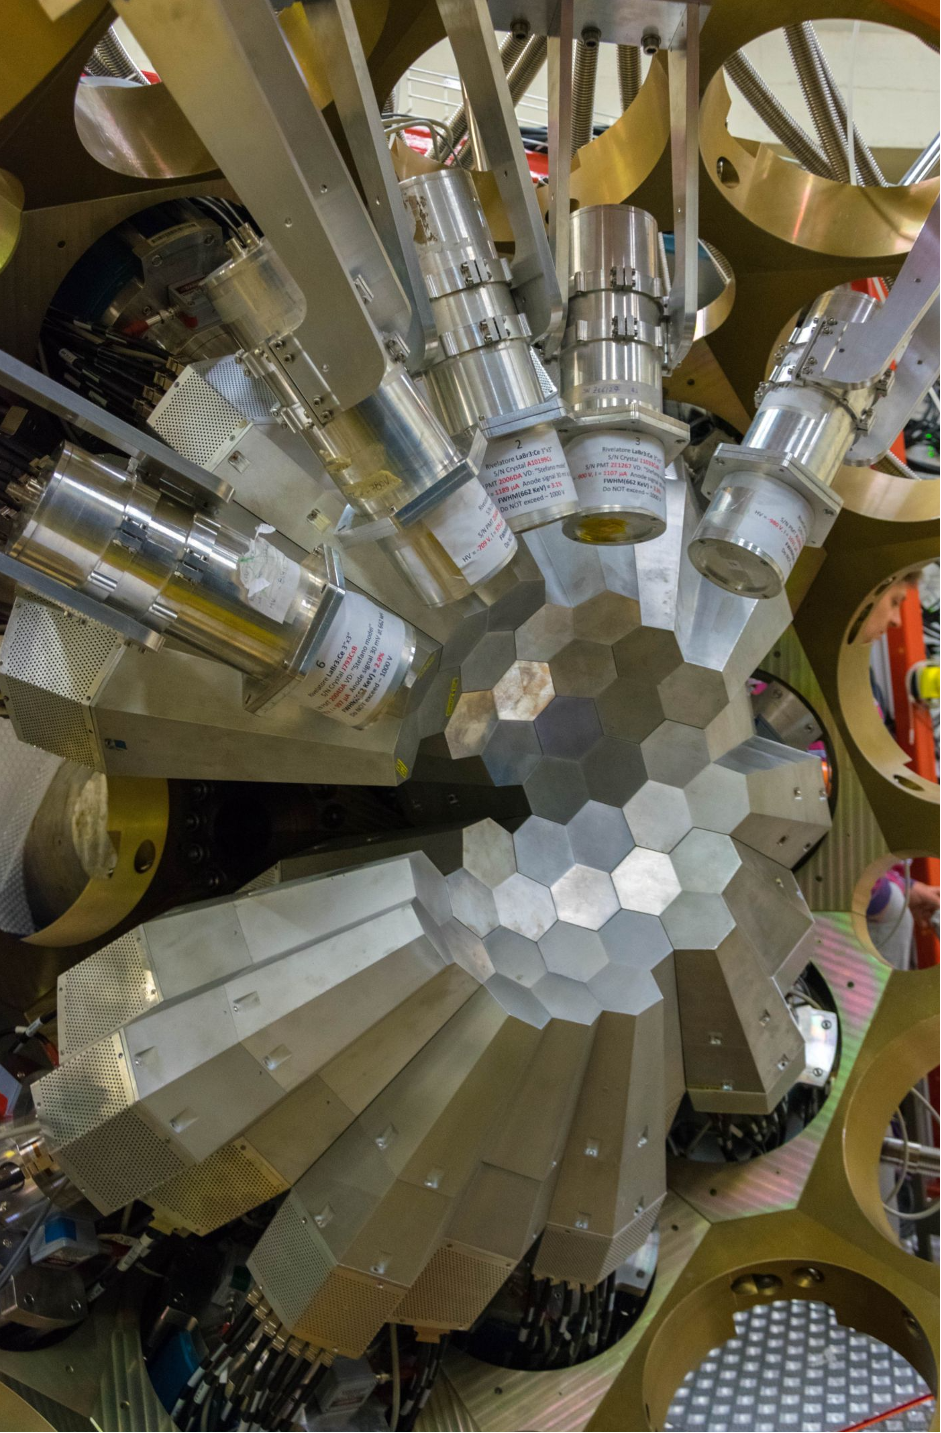
\includegraphics[width=0.5\linewidth]{graphics/AGATA_LNL.png}
    \caption{The AGATA gamma-ray tracking array installed at INFN-LNL.}
    \label{fig:AGATA_LNL}
\end{figure}

At \textbf{NLC-CCB} (Krakow) two long (lasting few weekends each) experiments were performed, with the use of 560 hours of high energy proton beams. 

At \textbf{NLC-SLCJ} (Warsaw), six supported experiments were carried out, using 1744 hours of beam time.

Only \textbf{INFN-LNS} has not delivered any access time, as it is under re-construction.

\subparagraph{Task 2.2: Radioactive Ion Beams} \mbox{}

%\todo{Briefly explain the progress of the task in context to the DoA.}

Period 2 was also very busy for the Radioactive Ion Beam facilities of Task 2.2. Four facilities have supported 82 experiments in this period, providing almost 6000 hours of RI beams. 

At the \textbf{GANIL-SPIRAL2} facility two projects received Transnational Access during P2, focusing on Nuclear Physics investigations on light radioactive nuclei and exploiting 224 hours of RI beams.

The RI beams at \textbf{GSI/FAIR} are delivered to the nuclear and astrophysics community (NUSTAR). During the P2 period, fourteen user projects have been supported by Transnational Access. 1248 hours of radioactive ion beams were provided. Within these experiments, different setups and parts of the facility were used, such as the experimental storage ring ESR, the R3B experiment, the DESPEC detector setup, the FRS itself, the FRS Ion Catcher and the EXPERT detector. 

%Experiments using FRS recorded a comprehensive dataset for projectile-fragmentation products (Z = 82 to 89) from 238U on a Be target, providing essential data to refine fragmentation models and support future NUSTAR experiments. ESR has been used for investigating the rare double-gamma decay mode in 0$^+$$\rightarrow$0$^+$ transitions, this study measured isolated double-photon decays in $^{72}$Ge, and compared the two-photon decay in $^{98}$Zr and $^{98}$Mo to assess whether enhanced transition rates depend on nuclear structure and measures of de-excitation probabilities over a wide energy range in excited $^{238}$U and $^{239}$U. For the first time, simultaneous measurements of fission, gamma, and multi-neutron emission (up to three neutrons) were achieved in a storage ring setting. R3B setup has been used for commissioning of key detectors (CALIFA, Si-tracker FOOT, NeuLAND). Cross-section measurements for (p,pd) reactions on various carbon isotopes were performed indicating the presence of strongly correlated neutron-proton pairs, with quasi-deuteron behavior influencing nucleon “dressing” in the nuclear medium. DESPEC gathered spectroscopic data around N=126 shell closer, a critical region for r-process nucleosynthesis, where new level schemes and transition probabilities help benchmark models describing the interplay of single-particle orbitals and collective excitations in heavy nuclei relevant for the astrophysical sites. FRS Ion Catcher has been used in three different experiments. A proof-of-principle study using slowed-down uranium beams in a Cryogenic Stopping Cell demonstrated that multi-nucleon transfer (MNT) reactions can produce neutron-rich isotopes (A $\approx$ 160–250). MNT products were successfully extracted and identified with the MR-TOF mass spectrometer, paving the way for future RIB production at Super-FRS. Also focusing on exotic nuclei from Br to Rh, this study addresses issues such as isospin symmetry breaking, the Wigner effect, and unexpected mass discrepancies (e.g., $^{70}$Br). The FRS Ion Catcher, combined with a $^{107}$Ag fragmentation beam and SIS-18 accelerator mode, delivered precise mass measurements, essential for validating nuclear models and rp-process calculations. EXPERT detector using a $^9$C beam, the experiment probes Thomas-Ehrman shifts in mirror pairs (e.g., $^5$H-$^5$Be, $^6$H-$^5$B, $^7$H-$^7$C) and measures decay energies, widths, and half-lives (down to picoseconds) via multi-particle angular correlations. Upgraded high-rate tracking detectors have enabled high-statistics data collection, allowing for improved measurements of nuclear state widths and the identification of novel multi-proton decay mechanisms.

At \textbf{JYFL} a total of six supported experiments were carried out using 888 hours of beam time access. %through Transnational Access during EURO-LABS P2. 

At the \textbf{CERN/ISOLDE} facility, 64 projects received Transnational Access during P2, focusing on Nuclear Physics investigations, and using 3604 hours of beam time.

\textbf{LNL/LNS} and \textbf{ALTO} had no Radioactive Ion Beams projects receiving Transnational Access during P2.

\subparagraph{Task 2.3: Neutron Beams} \mbox{}

%\todo{"Briefly explain the progress of the task in the context to the DoA"}

In P2, four neutron beam facilities supported 11 project, providing altogether more than 700 hours of neutron beams.

At CERN's \textbf{n\_TOF} facility, seven projects were granted Transnational Access during the EURO-LABS P2 phase, focusing on various nuclear physics investigations and exploiting 271 hours of beam.

At \textbf{CLEAR-CNA} one project using neutron beams was supported, with 48 hours of beam provided.

At the \textbf{ALTO} facility, one project using 72 hours of neutron beams from the LICORNE facility was supported.

At \textbf{GANIL-SPIRAL2} the NFS facility offered 328 hours of neutron beam to 2 projects.

\subparagraph{Task 2.4: Theoretical Support} \mbox{}

%\todo{Briefly explain the progress of the task in context to the DoA.}

Theoretical support for experimental activities was enhanced in P2 following two subtasks. 

WP 2.4.1 enables in-person TA to the European Centre for Theoretical Studies in Nuclear Physics and Related Areas (ECT*, Trento). During P2, ECT* hosted 30 workshops and one Doctoral Training Program (DTP), following calls for proposals in the spring and summer of  2023 and 2024. Calls are made through the ECT* website (\url{https://www.ectstar.eu}) and the extensive mailing list of ECT* associates. In addition, the ECT* Director and the Scientific Board actively solicit proposals to ensure a balanced annual program.

Among the successful proposals, the Scientific Board, which serves as User Selection Panel for EURO-LABS, selected for P2 10 workshops and the 2024 DTP.  A highlight was the DTP, which introduced students from different backgrounds in nuclear physics and astrophysics to the current state of the art in the field of nuclear astrophysics, regarding in particular new constraints on the equation of state of neutron-rich matter from nuclear theory, experiments, and observations, core-collapse supernovae as the birthplace of neutron stars, and mergers and gravitational waves as probes of the neutron-star interior. 

In the P2 period, ECT* provided access to 105 EURO-LABS users, using 479 Access Units (i.e. days spent by users in ECT*). In addition, the Scientific Board has selected EURO-LABS activities for the remainder of 2025, promoting workshops on several hot topics in nuclear physics.  
Among future activities, a highlight is a workshop in support of the Virtual Access provision in WP 2.4.2. 


WP 2.4.2 provides access to theoretical tools through the virtual-access (VA) infrastructure Theo4Exp. The service has been available since 1 February 2024 at \url{https://institucional.us.es/theo4exp}. Its opening to users has been posted in the EURO-LABS webpage and in social media, as well as distributed widely via mailing lists. The infrastructure consists of three installations: MeanField4Exp at IFJ PAN Kracow, Reaction4Exp at University of Sevilla, and Structure4Exp at University of Milano. The link to each installation can be easily found in the main webpage. User access to the installations is provided by the application \url{https://iam-eurolabs.ijclab.in2p3.fr/login}, which has been developed by WP5 of the present EURO-LABS project. This application ensures access to any researcher affiliated with a scientific institution via either eduGAIN (\url{https://edugain.org/}) or ORCID (\url{https://orcid.org/}).
An International Review Panel (IRP) meets every year to review and validate the progress made on the VA infrastructure and its three installations. The IRP is composed by P. Bednarczyk (IFJ-PAN, Chairperson), A. Moro-Mu\~noz (University of Seville), E. Vigezzi (INFN-Milano), K. Rusek (University of Warsaw), I.J. Thompson (Lawrence Livermore National Laboratory, LLNL), and A. Gargano (INFN-Napoli). Two meetings have been held in the reporting period P2, on 20th September 2023 and 10th October 2024. An article about Theo4Exp has appeared in the first 2025 issue of Nuclear Physics News 
(\url{https://www.tandfonline.com/doi/epdf/10.1080/10619127.2025.2454884}). 
A hands-on workshop, aimed at an optimal use of the Theo4Exp installations, is scheduled for July 2025 at ECT* (\url{https://www.ectstar.eu/workshops/theory-service-for-the-low-energy-nuclear-physics-community-a-hands-on-workshop/}).

In P2 13 projects (virtual services) were offered and realized by 188 remote users. In total 1915 Access Units (counted as each started hour of active use of the virtual service) were provided . These numbers are almost twice higher as estimated for the whole duration of the project.


\subparagraph{Task 2.5: Service Improvements } \mbox{}

%\todo{Briefly explain the progress of the task in context to the DoA.}

This task is divided into 5 different activities. A short summary of the latest progresses is provided below.

WP2.5.1 Streamlined and remote access: 

a) In the Streamlined Access part of the subtask, the offer of facilities providing beam for nuclear physics research within the WP2 package is presented in a more uniform and detailed way  through the website (still under construction) \url{https://www.slcj.uw.edu.pl/en/tna-euro-labs/}. Each facility has its own subpage with a menu that provides easy access to specific information, such as: site details, list of available infrastructures and beams, beam time schedule, application submission deadlines and details, meeting dates of Program Advisory Committies, total number of access units in use and still available, access procedures, details about the TNA support and the application process, and a list of publications. 

b) The Remote Access part of the subtask aims to provide improved remote access to EURO-LABS institutions (i.e., any kind of accessibility to experimental operation from outside of experimental areas, for locals experts and external participants). The main goals are to minimise required access to experimental areas and travel time for on-call experts, thus maximising external participation, and standardise generally-endorsed approaches and procedures. This subtask is divided into three main categories: i) the development of a user-friendly database to disseminate information on remote-access tools currently in use at EURO-LABS facilities, ii) the implementation of new/improved remote-access tools at EURO-LABS facilities, and iii) provide training opportunities to the community. The completion of part i) was reported in EURO-LABS project milestone M12 in February 2024. The database is fully operational (available here: \url{https://eurolabs-remote.gsi.de/}) and the collection of further information to expand the content is underway. A set of tools to provide remote control of the experimental irradiation setup are being implemented at the PARTREC facility, with the aim of minimising the amount of personnel needed on-site for guest research groups and/or paying customers of the PARTREC cyclotron.
To avoid potential security issues, users will not get direct access to the irradiation control system. Rather, they will receive access (via VPN) to an interface PC connected to the (less privileged) internal network.
A Python server running in the irradiation control PC parses the user’s input, and translates them into operations for the irradiation control system written in Labview, via the ActiveX interface. The server code will be open sourced in the near future.

With the aim of advertising the "Remote Handling" database, a half-day workshop has been organised as a satellite meeting to the "VIIth Topical Workshop on Modern Aspects in Nuclear Physics" conference on Feb. 4th, held in Bormio (Italy). 


WP2.5.2 Targets for high intense beams: A database containing information on the preparation and characteristics of the targets available at the participating institutions, as well as those newly developed as part of this subtask, has been completed. In particular, with the post-docs hired with EUROLABS funds at INFN-LNS and at GANIL, we collected information on the produced targets, their characteristics and manufacturing techniques from the collaborating institutions and the literature. The first version of this database is now ready and will be made public in the coming months via a user-friendly application.

WP2.5.3 Biomedical application (FLASH@EURO-LABS): Air-filled Farmer-type ionization chambers are widely used as standard detectors for absolute dosimetry in clinical settings. However, under Ultra-High-Dose-Rate (UHDR) conditions, these chambers experience significant recombination effects, resulting in high uncertainties in dose measurements.
The progress in this task was in 3 different topics: 1. Development and Benchmarking of a Numerical Model for Farmer-Type Ionization Chambers (cf. Fig.~\ref{fig:FLASH1}); 2. Application of the Developed Numerical Model: Evaluating the Reliability of the TM31023 Detector for Carbon Ion FLASH Applications; 3. Improvement of Dosimetry Uncertainty at Clinical Facilities. Results are summarized in the report of MS14.


\begin{figure}[!h]
    \centering
    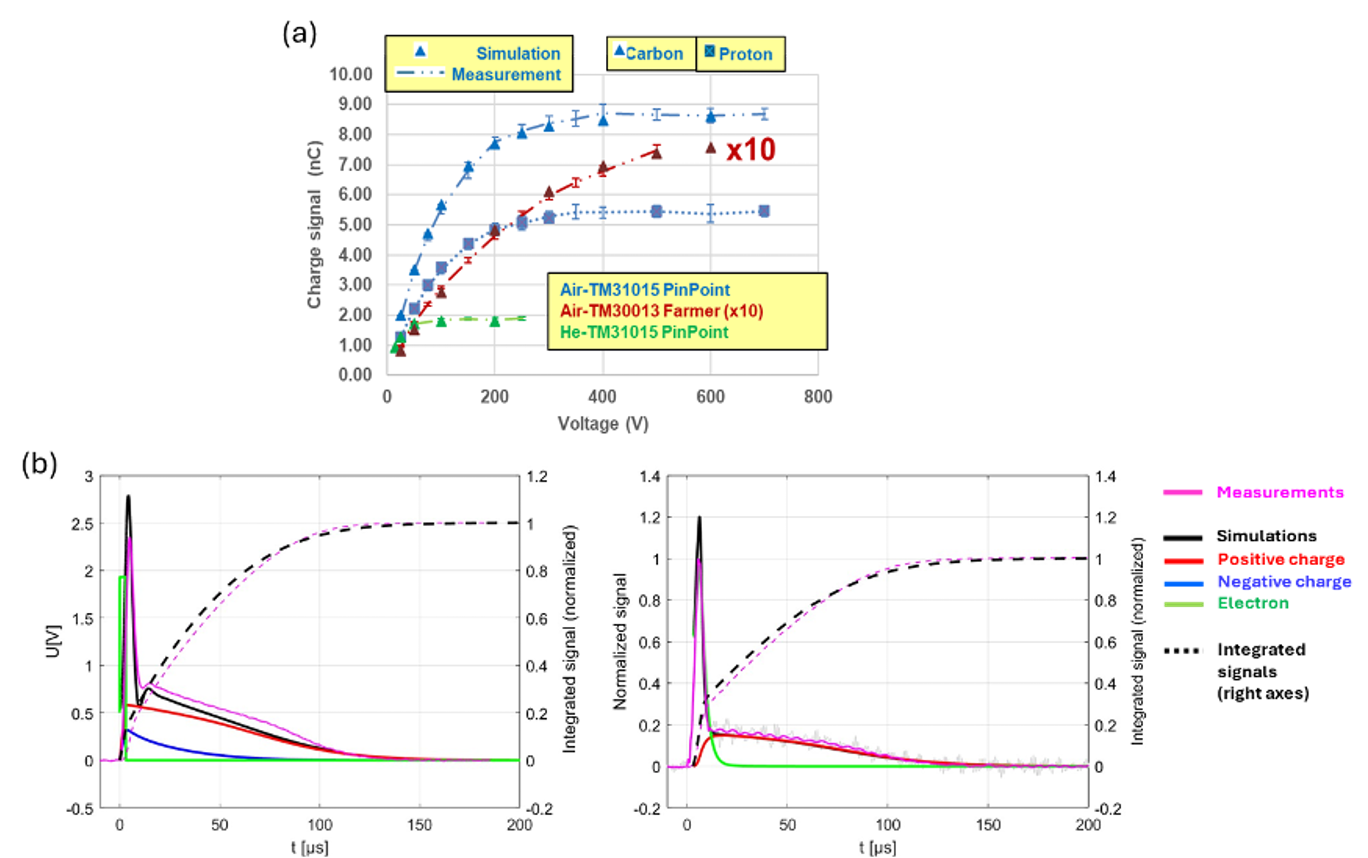
\includegraphics[width=1.0\linewidth]{graphics/FLASH1.png}
    \caption{Comparison of simulation and experimental data for FLASH dosimetry:
(a) Saturation curves of 3 different ionization chambers irradiated with protons at ultra-high dose rate at HIT in Heildeberg. (b) Time-resolved signals of the ionization chamber, whose integral corresponds to the charge collected by the electrometer, measured using a pulsed LINAC at Universitätsklinikum Gießen und Marburg (UKGM) at ultra-high dose rate. The signals from air-filled and nitrogen-filled Farmer chambers exhibit distinct differences in shape. This variation arises from the absence of electronegative molecules, such as oxygen, in the nitrogen-filled chamber, which prevents electron attachment.
}
    \label{fig:FLASH1}
\end{figure}

WP2.5.4 Improving Ion Beam services in variety and stability (ERIBS): The project has been divided into two separate parts to achieve the objectives. Part 1 focuses on extending the ion beam selection and intensities to allow new projectile-target combinations and/or make low-cross section reaction studies possible. Part 2 focuses on developing online beam monitoring to maintain the requested beam intensity. In Part 1 the main progress was in the MIVOC service and technology transfer. In Part 2 progress was done in optical emission spectroscopy and online beam intensity monitoring.

WP2.5.5 Optimal employment of traveling gamma detectors (INTRANS): The INTRANS (Instrumentation and Training for Nuclear Spectroscopy and Reaction Dynamics) subtask has organized and/or sponsored a series of events since September 2023, including: Two AGATA Analysis workshops; InTraNS Workshop; Gamma Detectors Hands-on Training on operation, test and repair of Hyper Pure Ge Detectors; InTraNS Training Workshop on Coulomb Excitation (see MS16). 

The work in all of the Service Improvements tasks is progressing according to the plan and shall be finished by the Month 36 of the EURO-LABS project.


\subsubsection*{Main Results and Achievements}

%\todo{Briefly summarise the main results and achievements of the DoA in context of the DoA.}

Progress in the TA offer in Tasks 1-3 is described above. 

Concerning Task 2.4, 
the main achievement was the opening to external users, in February 2024, of the Virtual Access facility Theo4Exp. All three components of Theo4Exp have implemented theoretical tools for the evaluation of experimental data. MeanField4Exp at IFJ PAN KraKow now offers mean-field predictions for the evolution of nuclear shape with angular momentum, as well as the effects of deformation and shape on single-particle and potential energies. Reaction4Exp, now online at University of Sevilla, enables the calculation of Coulomb breakup, elastic and inelastic scattering, and transfer reactions. Structure4Exp at University of Milano provides properties like masses and radii for ground and excited nuclear states from self-consistent mean-field methods and the Shell Model. In addition, collaborations between theorists and experimentalists were stimulated by 10 workshops and an advanced school hosted by ECT* (Trento), covering various aspects of nuclear structure, reactions and astrophysics, as well as strong and weak interactions, fundamental symmetries, high-power lasers, and machine learning.

The main achievements for task 2.5 in the P2 period are: i) the delivery of a new website in WP2.5.1; ii) a set-up for reduction and deposition in one-step of rare earth targets in WP2.5.2; iii) the reduction of dosimetry uncertainty to <0.15\%, significantly improving accuracy, in proton therapy centers using Farmer-type ionizing chambers for FLASH in WP2.5.3; iv) the use of optical emission spectroscopy as a real-time monitoring to provide early indications about plasma instabilities in ERIBS; v) the success of the INTRANS workshop, to the point that the INTRANS steering committee decided to hold an additional workshop towards the end of the EURO-LABS contract.





\subsubsection*{Deviations and Corrective Actions}
\label{sec:wp2-deviations}
There are two deviations - one positive, the other negative. The "positive" deviation of the project is that many TA facilities are delivering much more Access Units that planned, some of them already delivered more AU then declared for the whole project. The extra cost of the beam time is covered by the own facilities budget. So no corrective action is required.
The "negative" deviations from the originally planned schedule is slower spending, in some of the WP2 facilities, of the T\&S support. As the corrective action discussions of the EURO-LABS Steering Committee with the Facility Coordinators and corresponding UPS have started. As the result some simplifications of the ministrative procedures for the reimbursement are planned.  

% \todo{Briefly summarise any deviations and performed corrective actions of the DoA in context of the DoA.}

\subsubsection*{Milestones and Deliverables}
In the P2 reporting period, WP2 had five milestones to submit, which have been fully achieved.
{\fontsize{9}{11}\selectfont
\begin{center}
  \begin{tabular}[t]{!{\color{mygray}\vrule}p{0.10\linewidth}!
  {\color{mygray}\vrule}p{0.60\linewidth}!
  {\color{mygray}\vrule}p{0.20\linewidth}!{\color{mygray}\vrule} } \hline
    \rowcolor{mycyan} & {\bf Title} & {\bf Status} \\ \hline
    \cellcolor{mycyan}{\bf MS8}: &Calls for proposals to be hosted at ECT*&  Achieved - \href{https://web.infn.it/EURO-LABS/wp-content/uploads/2024/05/EURO-LABS_MS8-Final-1.pdf} {link}  \\ \hline
    \cellcolor{mycyan}{\bf MS10}: & Contracted personnel for Theo4Exp VA in place and first codes available for users in the virtual facility & Achieved - \href{https://web.infn.it/EURO-LABS/wp-content/uploads/2024/05/EURO-LABS_MS10_The4Exp_02_2024_FINAL-1.pdf}{link} \\ \hline    
    \cellcolor{mycyan}{\bf MS12}: & Completed database containing selected features of remote-access toolkit & Achieved - \href{https://web.infn.it/EURO-LABS/wp-content/uploads/2024/05/EURO-LABS_MS12-Report-RemoteAccess_Final.pdf}{link} \\ \hline 
    \cellcolor{mycyan}{\bf MS14}: & Reports on FLASH detectors for different facilities & Achieved - \href{https://web.infn.it/EURO-LABS/wp-content/uploads/2024/05/EURO-LABS_MS14_Report.pdf}{link} \\ \hline 
    \cellcolor{mycyan}{\bf MS16}: & 	Organisation of hands-on workshops and training schools & Achieved - \href{https://zenodo.org/records/15039933}{link} \\ \hline 
  \end{tabular}
\end{center}
}

\subsubsection*{Project Meetings}
\begin{table}[H]
    \centering
    \caption{Summary of WP2 meetings and discussed subjects.}

    \begin{tabularx}{\textwidth}{|c|p{0.32\linewidth}|x|} \hline
        \rowcolor{mycyan}
        \textbf{Date} & \textbf{Meeting \& Place} & \textbf{Subject} \\ \hline
        2023-10-09 & WP2 Task Leader's meeting in Krakow&Regular meeting \& progress report \\ \hline 
        2023-10-10 & General WP2 collaboration meeting in Krakow& Status of the project \& progress report \\ \hline         
        2024-08-26 & WP2.4 Collaboration meeting at the Zakopane conference & Status of the Theo4Exp VA facility \\ \hline
        2024-10-28 & WP2 Task Leader's meeting  at CERN & Regular meeting \& progress report \\ \hline
        2024-10-30 & General WP2 collaboration meeting at CERN& Status of the project \& progress report \\ \hline
        2024-11-5 & WP2 Collaboration meeting at the SSNET24 conference in Orsay &  Status of the project \& progress report \\ \hline  
        2024-09-25 & WP2.5 Collaboration meeting at the Bormio conference & Service improvements status \& progress report \\ \hline
    \end{tabularx}
    \label{tab:meetings}
\end{table}

In addition several ad-hoc meetings with the facility coordinators and task leaders were organized via zoom, when it was necessary. 

%  {\color{mygray}\vrule}p{0.40\linewidth}!







%%%%%%%%%%%%%%%%%%%%%%%%%%%%%%%%%%%%%%%%%


